Das Experiment dient dazu, die physikalischen Gesetze des Luftwiderstand zu erarbeiten und zu erlernen. 

\subsection{Aufbau des Experiments}

Für das Experiment wurden folgende Mittel verwendet:

\begin{itemize}
	\item 1 Entfernungsmesser
	\item 6 Testobjekte in Form von Papierkegel
	\begin{itemize}
		\item Grundfläche Kegel: \(132.736 cm^2\)
		\item Gewicht je Kegel: \(1.51 \pm 0.004g \)
	\end{itemize}
	\item 1 Rechner zur Aufzeichnung und Speicherung der Ergebnisse des Entfernungsmesser
	\begin{itemize}
		\item Betriebssystem: Windows 10 64 bit
		\item Aufzeichnungssoftware: Logger Pro (Trial)
	\end{itemize}
\end{itemize}

Diese wurden wie in der Abbildung \ref{fig:expsetup} angeordnet.



\begin{figure}
	\center
	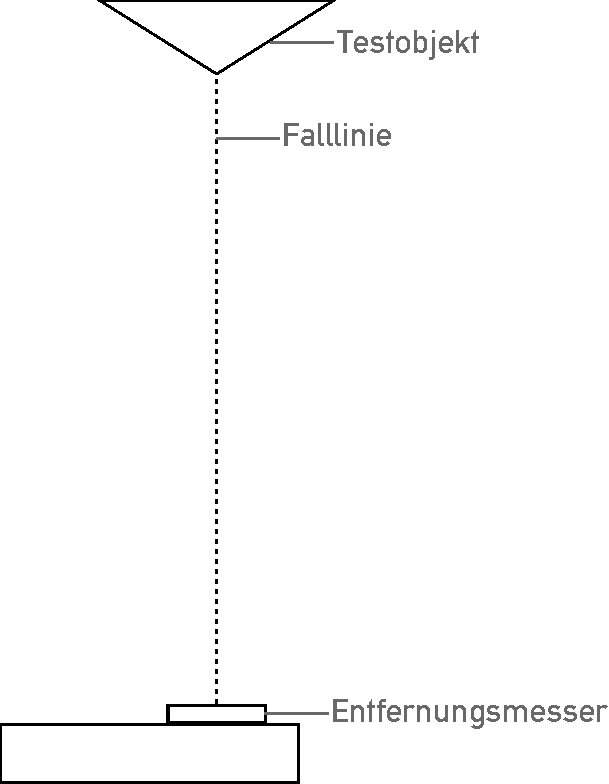
\includegraphics[width=5cm]{diagrams/experiment_aufbau}\caption{\label{fig:expsetup} Aufbau des Experiments}	
\end{figure}



\subsection{Ablauf des Experiments}


Es gab 5 Durchläufe des Experiments. Bei jedem Durchlauf wurden 1 oder mehrere Kegel 



\subsection{Versuchtes weiteres Experiment}

Um weitere Messergebnisse zu erhalten, wurde versuchsweise ein weiteres Experiment durchgeführt. Da dabei kein Entfernungsmesser verfügbar war, musste auf andere Mittel zurückgegriffen werden. Das zusätzliche Experiment beinhaltete die Komponenten welche auf der Abbildung \ref{fig:addexp} zu sehen sind. Das Experiment wurde gefilmt und bei der Auswertung konnte die Position des Kegels vom Messstab abgelesen und mit der Zeit des Videos abgeglichen werden.

Die Ergebnisse wurden jedoch nicht zur Analyse beigezogen da sie zu ungenau waren und somit das Endergebnis verfälscht hätten.

\begin{figure}
	\center
	\includegraphics{diagrams/aufbau2}
	\caption{\label{fig:addexp} Aufbau des zusätzlichen Experiments}
\end{figure}